\id{МРНТИ 65.63.33}

{\bfseries СҮТ САРЫСУЫ НЕГІЗІНДЕ СҮТҚЫШҚЫЛДЫ СУСЫНДАРДЫҢ САПАСЫН ЖЕТІЛДІРУ}

{\bfseries \textsuperscript{1}А.А.
\begin{figure}[H]
	\centering
	
\includegraphics[width=0.8\textwidth]{media/pish4/image1}
	\caption*{}
\end{figure}

\textsuperscript{1}Э.К.
\begin{figure}[H]
	\centering
	
\includegraphics[width=0.8\textwidth]{media/pish4/image1}
	\caption*{}
\end{figure}

\textsuperscript{1}Ш.А.
\begin{figure}[H]
	\centering
	
\includegraphics[width=0.8\textwidth]{media/pish4/image1}
	\caption*{}
\end{figure}


{\bfseries \textsuperscript{2}К.А.
\begin{figure}[H]
	\centering
	
\includegraphics[width=0.8\textwidth]{media/pish4/image1}
	\caption*{}
\end{figure}

\textsuperscript{1} М.О.
\begin{figure}[H]
	\centering
	
\includegraphics[width=0.8\textwidth]{media/pish4/image1}
	\caption*{}
\end{figure}


\textsuperscript{1}Алматы технологиялық университеті АҚ, Алматы,
Қазақстан,

\textsuperscript{2}Қазақ ұлттық аграрлық зерттеу университеті, Алматы,
Қазақстан

{\bfseries \textsuperscript{\envelope }}Корреспондент-автор:
\href{mailto:elmiraasembaeva@mail.ru}{\nolinkurl{elmiraasembaeva@mail.ru}}

\begin{enumerate}
\def\labelenumi{\arabic{enumi}.}
\item
  https://orcid.org/ 0009-0002-8382-7726
\item
  \url{https://orcid.org/0000-0001-7964-7736}.
\item
  \href{https://orcid.org/0000-0001-7258-746X}{https://orcid.org/0000-0003-3209-6855}
\item
  https://orcid.org/ 0000-0003-0588-6659
\item
  https://orcid.org/0000-0001-5767-5154.
\end{enumerate}

Ғылыми-техникалық дамудың қазіргі кезеңінде шикізатты кешенді пайдалану
және қалдықсыз технологияларды жетілдіру басты бағыт болып табылады.
Экологиялық жағдайды ескере отырып, табиғи ресурстарды үнемдеу маңызды.
Сүт өндірісінде сүт тапшылығы мәселесіне байланысты сарысу сүт
компоненттерінің қосымша көзі ретінде қолданылып, функционалдық өнімдер
жасау үшін ерекше мәнге ие. Сарысудың көмірсулар мен ақуыздық құрамының
артықшылығы - бұл негізгі шикізат тапшылығын шешудің тиімді әдісі.

Зерттеудің мақсаты сүт сарысуынан үйеңкі шәрбаты қосылған сүтқышқылды
сусын әзірлеу және оның сапасы мен қауіпсіздігін зерттеу. Алынған сарысу
сусынының органолептикалық (түсі, иісі, дәмі, консистенциясы),
физика-химиялық (қышқылдығы), реологиялық (синергетикалық қабілеті) және
микробиологиялық көрсеткіштері (МАжФАнМС, ІТТБ, \emph{Salmonella}
туысының бактериялары, \emph{Staphylococcus aureus,} ашытқылар мен
зеңдер) бойынша талдау жүргізілді. Органолептикалық, физика-химиялық
және микробиологиялық көрсеткіштері бойынша жүргізілген зерттеулер
нәтижесінде үйеңкі шәрбаты қосылған ұсынылатын сарысу сусынының сапасы,
тағамдық және биологиялық құндылығы жоғары екені анықталды.

Сүт сарысуынан үйеңкі шәрбатын қосып алынған сүтқышқылды сусынның дәмі
жағымды, нәзік, орташа тәтті болды. Сүтқышқылды сусынның сақтау мерзімі
(4±2) °C температурада 7 тәулік. Алынған сүт сусыны асқазан-ішек
жолдарындағы бактериялық және саңырауқұлақ инфекцияларының алдын алу
үшін пайдалы болады, сонымен қатар жалпы мақсаттағы асхана сусыны
ретінде қолдануға болады. Төмен калориялы сүтқышқылды сусындар сүт
өнімдерінің ассортиментін кеңейтіп, тұтынушылардың сұранысын арттыруға
ықпал етеді.

{\bfseries Түйін сөздер:} сүт сарысуы, сүтқышқылды сусын, үйеңкі шәрбаты,
минералды заттар, сақтау мерзімі, микробиологиялық көрсеткіш.

{\bfseries УЛУЧШЕНИЕ КАЧЕСТВА КИСЛОМОЛОЧНЫХ НАПИТКОВ}

{\bfseries НА ОСНОВЕ СЫВОРОТКИ}

{\bfseries \textsuperscript{1}А.А. Турганбаева, \textsuperscript{1}Э.К.
Асембаева\textsuperscript{\envelope }, \textsuperscript{1}Ш.А.Абжанова,}

{\bfseries \textsuperscript{2}К.А. Мырзабек, \textsuperscript{2}М.О.
Кожахиева}

\textsuperscript{1}Алматинский технологический университет, Алматы,
Казахстан,

\textsuperscript{2}Казахский национальный аграрный исследовательский
университет, Алматы, Казахстан,

e-mail:
\href{mailto:elmiraasembaeva@mail.ru}{\nolinkurl{elmiraasembaeva@mail.ru}}

На современном этапе научно-технического развития главным направлением
является комплексное использование сырья и совершенствование безотходных
технологий. Учитывая экологическую обстановку, важно экономить природные
ресурсы. Из-за проблемы дефицита молока в молочном производстве
сыворотка используется в качестве дополнительного источника компонентов
молока и имеет особое значение для создания функциональных продуктов.
Преимущества углеводного и белкового состава сыворотки заключаются в
том, что она представляет собой эффективный метод решения проблемы
дефицита основного сырья.

Целью исследования является разработка кисломолочного напитка из
сыворотки с добавлением кленового сиропа и исследование его качества и
безопасности. Проведен анализ полученного сывороточного напитка по
органолептическим (цвет, запах, вкус, консистенция), физико-химическим
(кислотность), реологическим (синергетическая способность) и
микробиологическим показателям (КМАФАнМ, БГКП, бактерии рода
\emph{Salmonella, Staphylococcus aureus,} дрожжи и плесень).
Исследования по органолептическим, физика-химическим и
микробиологическим показателям показали, что рекомендуемый сывороточный
напиток с кленовым сиропом имеет хорошее качество и высокую пищевую и
биологическую ценность.

Кисломолочный напиток, приготовленный из сыворотки с добавлением
кленового сиропа, имел приятный, нежный, умеренно сладкий вкус. Срок
годности кисломолочного напитка - 7 суток при температуре (4±2) °С.
Полученный молочный напиток будет полезен для профилактики бактериальных
и грибковых инфекций желудочно-кишечного тракта, а также может
использоваться в качестве универсального напитка на кухне.
Низкокалорийные молочные напитки расширяют ассортимент молочной
продукции и способствуют повышению потребительского спроса.

{\bfseries Ключевые слова:} молочная сыворотка, кисломолочный напиток,
кленовый сироп, минеральные вещества, срок годности, микробиологические
показатели.

{\bfseries IMPROVING THE QUALITY OF FERMENTED MILK DRINKS}

{\bfseries BASED ON WHEY}

{\bfseries \textsuperscript{1}А.А. Turganbaeva, \textsuperscript{1}E.K.
Assembayeva\textsuperscript{\envelope }, \textsuperscript{1}Sh.А.Abzhanova,}

{\bfseries \textsuperscript{2}К.А. Myrzabek, \textsuperscript{1}М.О.
Kozhakhiyeva}

\textsuperscript{1}Almaty Technological University, Almaty, Kazakhstan,

\textsuperscript{2}Kazakh National Agrarian Research University, Almaty,
Kazakhstan,

e-mail: elmiraasembaeva@mail.ru

At the present stage of scientific and technological development, the
main direction is the integrated use of raw materials and the
improvement of waste-free technologies. Considering the environmental
situation, it is important to save natural resources. Due to the problem
of milk shortage in dairy production, whey is used as an additional
source of milk components and is of particular importance for the
creation of functional products. The advantages of the carbohydrate and
protein composition of whey are that it is an effective method for
solving the problem of shortage of the main raw materials.

The aim of the study is to develop a fermented milk drink from whey with
the addition of maple syrup and to study its quality and safety. The
analysis of the obtained whey drink was carried out according to
organoleptic (color, odor, taste, consistency), physico-chemical
(acidity), rheological (synergetic ability) and microbiological
parameters (QMAFAnM, \emph{Escherichia coli}, bacteria of the genus
\emph{Salmonella, Staphylococcus aureus}, yeast and mold). Studies on
organoleptic, physical, chemical and microbiological parameters have
shown that the recommended whey drink with maple syrup is of good
quality and has high nutritional and biological value.

The fermented milk drink made from whey with the addition of maple syrup
had a pleasant, delicate, moderately sweet taste. The shelf life of the
fermented milk drink is 7 days at a temperature of (4±2) °C. The
resulting milk drink will be useful for the prevention of bacterial and
fungal infections of the gastrointestinal tract, and can also be used as
a universal drink in the kitchen. Low-calorie milk drinks expand the
range of dairy products and contribute to an increase in consumer
demand.

{\bfseries Keywords:} whey, fermented milk drink, maple syrup, minerals,
expiration date, microbiological indicators.

{\bfseries Кіріспе.} Бүгінгі таңда сүт өңдеу саласында шикізат тапшылығы
байқалуда, сондықтан сүт сарысуын толық көлемде пайдалану өндіріс
шығындарын төмендетіп, өнімнің бәсекеге қабілеттілігін арттыруға
мүмкіндік береді. Сүт сарысуын пайдалану немесе сүт компоненттерін
сарысудың құрамдас бөліктерімен ауыстыру арқылы сүт өңдеу кәсіпорындары
өз өндіріс шығындарын азайтып, жаңа өнімдер шығаруға және нарықтағы
бәсекеге қабілеттілігін арттыруға қол жеткізе алады.

Екіншілік сүт шикізатын, әсіресе сарысуды тиімді өңдеу сүт өнімдерінің
көлемін арттырудың маңызды мүмкіндігі болып табылады. Қазіргі уақытта
сүт өнеркәсібінің көпшілігінде ірімшік пен сүзбе өндірісінде екіншілік
өнім болып саналатын, құрамында шамамен 55\%-ға дейін сүттің құрғақ
заттары бар сарысуды тиімді өңдеу мәселесі толық шешілген жоқ. Бұл
қоршаған ортаға кері әсерін тигізіп, экологиялық қауіптердің артуына
себеп болуы мүмкін, өйткені сарысу тұрмыстық сарқынды сулардан 500-1000
есе көп ластау қабілетіне ие {[}1-3{]}.

Соңғы он жылда отандық және шетелдік зерттеушілер сарысу мен оның
құрамдас бөліктері негізінде әртүрлі өнімдер әзірледі, олардың негізгі
бөлігі сусындар {[}3-6{]}.

Сарысуды дәмдеуіштермен, хош иісті заттармен және басқа
толықтырғыштармен байыту тұтынушылар арасында танымал көптеген
сусындарды шығаруға мүмкіндік береді. Сарысуды ашыту процесі барысында
жеміс-жидек пен қант шәрбаттарын, арнайы бояғыштар мен дәмдеуіштерді,
сондай-ақ басқа құрамдас бөліктерді қосу арқылы оның дәмі мен пайдалы
қасиеттерін арттыруға болады.

Сарысу ақуыздары өздерінің тағамдық және биологиялық құндылығы жағынан
ең бағалы болып саналады, бұл оларды емдік-профилактикалық өнімдер үшін
перспективалы шикізатқа айналдырады. Бұл ақуыздар алмастырылмайтын
аминқышқылдарының толық спектрін қамтиды және аминқышқылдық құрамы
бойынша адамның физиологиялық қажеттіліктерін толық қанағаттандыратын
идеал ақуызға жақын келеді {[}7,8{]}. В тобы дәрумендерінің көп болуына
байланысты сарысудан дайындалған сусындар тұтастай алғанда адам ағзасына
күшейтетін әсер етеді {[}9{]}.

Сарысу сусындарының органолептикалық қасиеттерін жақсарту үшін тағамдық
қоспалар, оның ішінде функционалды қасиеттері бар өсімдік негізіндегі
қоспалар жиі пайдаланылады. Дәрілік өсімдіктердің сығындылары сусындарды
дәрумендермен және полифенолдармен байытады, олар иммундық жүйені
нығайтуға, физикалық және жүйкелік шаршауды жеңілдетуге, өміршеңдікті
арттыруға, холестерин деңгейін төмендетуге және қатерлі ісік қаупін
азайтуға көмектеседі {[}10{]}.

Үйеңкі шәрбаты -- қант, қызыл және қара үйеңкі ағаштарының шырынынан
алынатын тәтті шәрбат. Ол дайын тағамдарға қосымша ретінде және тәтті
тағамдардың рецептерінде компонент ретінде кеңінен қолданылады. Үйеңкі
шәрбатының басқа тәттілендіргіштерден басты артықшылығы -- оның
құрамында оксалаттар мен пуриндер өте аз, сондықтан ол тағамдық аллергия
тудырмайды. Сонымен қатар, үйеңкі шәрбаты бактерияға, диабетке қарсы
қасиеттерге ие, жүрек-тамыр жүйесінің жұмысын жақсартады және басқа да
пайдалы әсерлері бар. Шәрбат кальций, мырыш, темір, фосфор және калий
сияқты маңызды минералдарға бай. Оның құрамында В тобының барлық
дәрумендері, соның ішінде өте сирек кездесетін тиамин дәрумені де бар.
Сонымен қатар, термиялық өңдеу кезінде бұл өнім денсаулыққа зиян
келтірмейді {[}11-13{]}.

Сүт өнеркәсібінде өнімнің органолептикалық қасиеттерін жақсарту
мақсатында әртүрлі толықтырғыштар пайдаланылады. Осы тұрғыда, үйеңкі
шәрбатын қосу тиімді шешім болуы мүмкін. Үйеңкі шәрбатымен байытылған
өнім тек дәмді ғана емес, сонымен қатар қосымша пайдалы қасиеттерге де
ие болады. Таза үйеңкі шәрбаты -- бұл тек үйеңкі ағашының шырынынан
алынатын табиғи өнім. Ол қант, бояғыштар, жасанды хош иістендіргіштер,
консерванттар немесе басқа қоспаларсыз, тек табиғи органикалық
тәттілендіргіш болып табылады.

Осылайша, сарысу негізінде сусындар өндірісін дамыту және сүт
өнеркәсібінің осы саласындағы өнім ассортиментін кеңейту сарысуды
қосалқы өнім ретінде пайдаланатын кәсіпорын үшін маңызды әрі
экономикалық тұрғыдан тиімді болып табылады.

Зерттеудің мақсаты сүт сарысуынан үйеңкі шәрбаты қосылған сүтқышқылды
сусын әзірлеу және оның сапасы мен қауіпсіздігін зерттеу.

{\bfseries Материалдар мен әдістер.}Зерттеу нысаны ретінде сүзбе
өндірісінен алынған екіншілік шикізат -- сүт сарысуы алынды. Өсімдік
шикізаты ретінде Ресейде жасалған Пензалық үйеңкі шәрбаты пайдаланылды.

Сүтқышқылды сарысу сусыны дәстүрлі технология бойынша сүт сарысуы және
\emph{Lactobacillus delbrueckii subsp. bulgaric және Streptococcus
thermophilus} ұйытқы негізінде дайындалды.

Талдау жүргізу үшін екі үлгі әзірленді: бақылау үлгісі -- қоспасыз сүт
сарысуы сусыны; зерттелетін үлгі -- үйеңкі шәрбаты қосылған сүт сарысуы
сусыны.

Сүтқышқылды сусынның синергетикалық қабілеті центрифугалау әдісі арқылы
анықталды. Ол үшін 10 см\textsuperscript{3} ұйынды 15
см\textsuperscript{3} сыйымдылығы бар центрифуга пробиркасына құйылып,
белгіленген жылдамдықпен (2000 айн/мин) 5 минут бойы центрифугаланады.
Центрифугалау аяқталғаннан кейін бөлінген сарысу декантацияланып, көлемі
10 см\textsuperscript{3} болатын шыны градуирленген центрифуга
пробиркасына өлшенеді. Бөлінген сарысу мөлшері арқылы ұйындының ылғал
жоғалту қабілеті бағаланады. Нәтижелер 10 см\textsuperscript{3}
ұйындыдан алынған сарысу көлемімен (мл) көрсетіледі.

Титрлеу қышқылдығы MEMСT 3624-92 «Сүт және сүт өнімдері. Қышқылдықты
анықтаудың титриметриялық әдістері» стандартына сәйкес анықталды. Ол
Тернер градусымен есептеліп, соңғы нәтиже ретінде екі параллельді
өлшеудің орташа арифметикалық мәні алынды.

Зерттелген сусын үлгілерінің қауіпсіздігі төмендегідей көрсеткіштер
арқылы бағаланып, мемлекеттік стандартта бекітілген әдістер арқылы
талданды:

-- мезофильді аэробты және факультативті анаэробты микроорганизмдердің
саны (МАжФАнМС) MEMСT 10444.15-94;

-- ішек таяқшасы тобындағы бактериялар саны (ITTБ) MEMСT 31747-2012;

-- зеңдер мен ашытқылар MEMСT 10444.12-2013;

\begin{itemize}
\item
  \emph{Salmonella} туысының бактерияларын анықтау әдісі МЕМСТ
  31659-2012;
\end{itemize}

-- \emph{Staphylococcus aureus} МЕМСТ 30347-2016.

Сусын үлгілеріндегі минералды заттар құрамын, соның ішінде натрий,
калий, кальций, магний, мырыш, марганец мөлшерін атомды-адсорбционды
спектрометриялық әдіспен анықталды.

Зерттеу жұмыстары Алматы технологиялық университетінің «Тағамдық
биотехнология» кафедрасы мен «Тамақ қауіпсіздігі» ғылыми зерттеу
институтының зертханаларында жүргізілді. Тәжірибелік зерттеулер 3-5 рет
қайталанып, орташа арифметикалық мәндер алынды.

{\bfseries Нәтижелер және талқылау.}

Сарысудан сусындарды алу технологиясы қарапайым, арнайы жабдықты қажет
етпейді және кез келген сүт зауытында оңай жүзеге асырылады. Жалпы
алғанда, технологиялық процесс келесі операцияларды қамтиды: шикізатты
қабылдау және дайындау (4±2 °С); сарысуды тазарту; пастерлеу (90±2 °C,
t=5 минут) және қоспаны ашыту температурасына дейін (42±2 °C)
салқындату; ашыту (42±2 °C, t=6-8 сағат); салқындату (4±2 °С); дайын
шәрбатты араластыру; құю, орау және сақтау (4±2 °С).

Жұмыстың бастапқы кезеңінде өнімнің органолептикалық қасиеттерін
жақсарту мақсатында үйеңкі шәрбатын толықтырғыш және тәттілендіргіш
ретінде қолданудың оңтайлы мөлшерін анықтау үшін тәжірибелер жүргізілді.
Тәжірибе барысында үйеңкі шәрбатының 2,5\%, 5\% және 7,5\% үлестері
қосылған үлгілер дайындалды. Үйеңкі шәрбаты бар өнімдер тәтті дәмге ие
болды, оның қарқындылығы шәрбаттың мөлшеріне байланысты өзгеріп отырды.
2,5\% үйеңкі шәрбаты қосылғанда дәмі аздап тәтті болып, шәрбаттың дәмі
білінбеді. 5\% үйеңкі шәрбаты қосылған үлгіде дәмі тәтті, жағымды болып
шықты, бұл үлгі басқалардан ерекшеленіп, ең жоғары бағаға ие болды. Ал
7,5\% шәрбат қосылған үлгі тым тәтті болып, қышқыл сүттің дәмі мүлде
сезілмей қалды, бұл оның жалпы бағасын төмендетті. Осы мәліметтер
негізінде 5\% үйеңкі шәрбаты қосылған үлгі ең жақсы органолептикалық
қасиеттерге ие деп қорытынды жасауға болады. Бұл мөлшер оңтайлы болып
табылды.

Өндірілетін өнімнің сапасының маңызды көрсеткіші -- синерезис. Бұл
көрсеткіш ұйындының беріктігін және өнімнің тұтынушылық қасиеттерін
анықтайды.

Бұл жұмыста үйеңкі шәрбатының сүтқышқылды сусынның синергетикалық
қасиетіне әсері зерттелді. Зерттеу барысында 30 минуттық
центрифугалаудан кейін әр 5 минут сайын бөлінген сарысу мөлшері
есептелді. Бөлінген сарысу көлемі ұйындының ылғал жоғалту қабілетін
бағалауға мүмкіндік береді. Нәтижелер 10 см\textsuperscript{3} ұйындыдан
бөлінген сарысу көлемі (мл) арқылы анықталды. Зерттеу нәтижелері
1-суретте көрсетілген.

\begin{figure}[H]
	\centering
	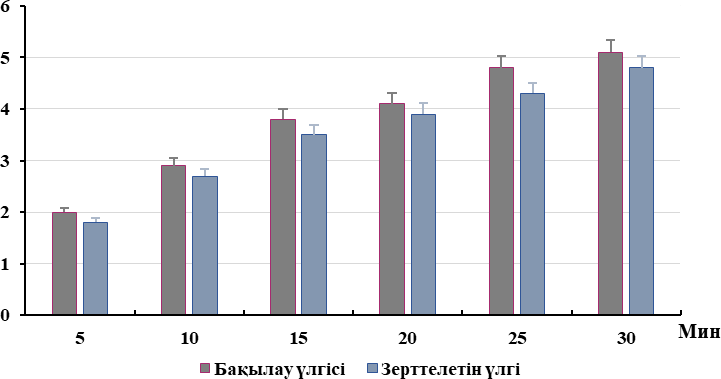
\includegraphics[width=0.8\textwidth]{media/pish4/image2}
	\caption*{}
\end{figure}


{\bfseries 1-сурет. Сарысудан алынған сусындардың синергетикалық қабілеті}

Алынған нәтижелерге сәйкес, зерттелетін үлгімен салыстырғанда бақылау
үлгісінде сарысудың көп мөлшері бөлінетіндігі байқалады. 30 минуттан
кейін бақылау үлгісінде --сарысу 5,2 мл бөлінсе, зерттелетін үлгіде --
4,7 мл бөлінді. Сарысудың аз бөлінуі оның бақылау үлгісіне қарағанда
ұзақ сақталатынын көрсетеді.

Өнімдердің сақтау мерзімін сақтау кезіндегі қышқылдық деңгейімен
анықтауға болады (1-сурет).

\begin{figure}[H]
	\centering
	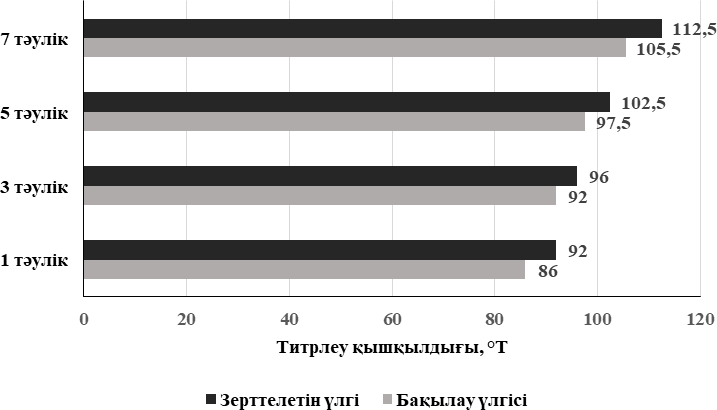
\includegraphics[width=0.8\textwidth]{media/pish4/image3}
	\caption*{}
\end{figure}


{\bfseries 2-сурет. Сарысудан алынған сусындардың қышқылдығы, °Т}

Бақылау үлгісінің бірінші тәуліктегі қышқылдығы -- 86°Т, ал зерттелетін
үлгінікі -- 92 °Т болды. Сақтаудың жетінші күні бақылау үлгісінің
қышқылдығы -- 105,5 °Т, ал зерттелетін үлгінікі -- 112,5 °Т дейін өсті.
Осылайша, алынған мәліметтерге сәйкес, сарысу негізіндегі сүтқышқылды
сусынының сақтау мерзімін (4±2) °C температурада 7 тәулік деп айтуға
болады.

\begin{figure}[H]
	\centering
	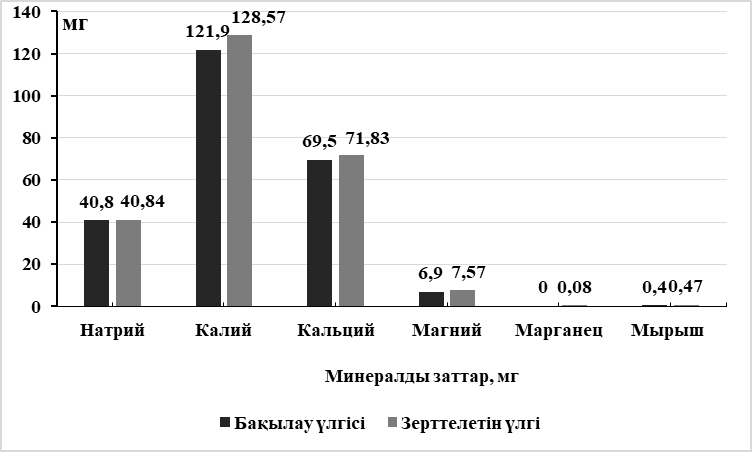
\includegraphics[width=0.8\textwidth]{media/pish4/image4}
	\caption*{}
\end{figure}


{\bfseries 3-сурет. Сүт сарысуынан алынған сусындардың минералдық құрамы}

Алынған талдау нәтижелерінен сүт сарысуына үйеңкі шәрбатын қосу арқылы
минералдық құрамын толықтыруға болатынын көруге болады. Марганец бақылау
үлгісінде болмады, ал зерттелетін үлгіде 0,08 мг болғанын көруге болады.
Марганец функционалдық ингредиенттердің D класына жатады және сүйек
қаңқасын құрайтын дәнекер тінінің синтезін қамтамасыз ету арқылы
остеопороздың алдын алуға белсенді қатысады. Мырыш А класына жатады және
қандағы инсулин деңгейін ұстап тұрумен байланысты функцияларды орындай
отырып, көмірсу алмасу процесіне қатысады {[}14{]}.

Микробиологиялық көрсеткіштері бойынша сүт сарысуынан жасалған сусын сүт
және сүт өнімдеріне қойылатын техникалық регламенттердің талаптарына,
сондай-ақ санитарлық-эпидемиологиялық қадағалауға (бақылауға) жататын
тауарларға қойылатын Бірыңғай санитарлық-эпидемиологиялық және
гигиеналық талаптарға сәйкес болуы керек. Алынған сусынның
микробиологиялық көрсеткіштері 1-кестеде келтірілген.

{\bfseries 1 - кесте. Сүт сарысуынан алынған сусынның микробиологиялық
көрсеткіштері}

% \begin{longtable}[]{@{}
%   >{\raggedright\arraybackslash}p{(\columnwidth - 10\tabcolsep) * \real{0.1728}}
%   >{\raggedright\arraybackslash}p{(\columnwidth - 10\tabcolsep) * \real{0.1671}}
%   >{\raggedright\arraybackslash}p{(\columnwidth - 10\tabcolsep) * \real{0.1291}}
%   >{\raggedright\arraybackslash}p{(\columnwidth - 10\tabcolsep) * \real{0.2352}}
%   >{\raggedright\arraybackslash}p{(\columnwidth - 10\tabcolsep) * \real{0.1507}}
%   >{\raggedright\arraybackslash}p{(\columnwidth - 10\tabcolsep) * \real{0.1451}}@{}}
% \toprule\noalign{}
% \endhead
% \bottomrule\noalign{}
% \endlastfoot
% \multirow{2}{=}{Көрсеткіштер} & \multirow{2}{=}{MAФАнMМ,
% КТБ/см\textsuperscript{3} (г), артық емес} &
% \multicolumn{3}{>{\raggedright\arraybackslash}p{(\columnwidth - 10\tabcolsep) * \real{0.5150} + 4\tabcolsep}}{%
% Рұқсат етілмеген өнімнің салмағы (г, см\textsuperscript{3}).} &
% \multirow{2}{=}{Ашытқы мен зеңдер, КТБ/см\textsuperscript{3} (г), артық
% емес} \\
% & & ІТТБ (колиформалар) & Патогенді микро- организмдер, соның ішінде
% 
% сальмонелла-лардың саны & Staphylococcus aureus \\
% НҚ бойынша рұқсат етілген шек & 1*10\textsuperscript{5} & 0,01 & 25 &
% 1,0 & рұқсат етілмейді \\
% Зерттелетін үлгі & 1,2*10\textsuperscript{3} &
% \multicolumn{3}{>{\raggedright\arraybackslash}p{(\columnwidth - 10\tabcolsep) * \real{0.5150} + 4\tabcolsep}}{%
% табылмады} & табылмады \\
% \end{longtable}

Алынған нәтижелерден алынған сусында ішек таяқшалары тобындағы
бактериялар, сальмонеллалар, \emph{Staphylococcus aureus, Listeria
L.monocytogenes}, ашытқылар мен зеңдер табылмады, ал мезофильді аэробты
факультативті анэробты микроорганизмдер мөлшері рұқсат етілген деңгейден
аспады, яғни 1,2*10\textsuperscript{3} КТБ/см\textsuperscript{3} болды.

{\bfseries Қорытынды}. Сүт сарысуынан үйеңкі шәрбатын қосып алынған
сүтқышқылды сусынының дәмі жағымды, нәзік, орташа тәтті болды.
Сүтқышқылды сусынның сақтау мерзімі (4±2) °C температурада 7 тәулік.
Төмен калориялы сүтқышқылды сусындар сүт өнімдерінің ассортиментін
кеңейтіп, тұтынушылардың сұранысын арттыруға ықпал етеді.

{\bfseries Әдебиеттер}

1.Габриелян Д.С., Грунская В.А. Ресурсосберегающая технология
обогащенных кисломолочных напитков //Пищевая промышленность. - 2014.- №.
8. -С. 12-14.

2.Волкова Т.А. О роли продуктов из сыворотки //Молочная
промышленность.-2012. -№. 4. - С. 69.

~3. Rocha-Mendoza D. et al. Invited review: Acid whey trends and health
benefits //Journal of Dairy Science. - 2021.- Vol.104(2). Р. 1262-1275.
\href{https://doi.org/10.3168/jds.2020-19038}{DOI
10.3168/jds.2020-19038}

4. Oliveira G.A.R. et al. Benefits of thermosonication in orange juice
whey drink processing //Innovative Food Science \& Emerging
Technologies.-2022.- Vol75:102876.

\href{https://doi.org/10.1016/j.ifset.2021.102876}{DOI
10.1016/j.ifset.2021.102876}

5.Утебаева А.А. и др. Функциональные напитки на основе сыворотки с
экстрактом виноградной выжимки и фруктовым соком //Вестник Алматинского
технологического университета.- 2024. - Т. 145(3).- С. 26-38.
\href{https://doi.org/10.48184/2304-568X-2024-3-26-38}{DOI
10.48184/2304-568X-2024-3-26-38}

6. Айтжанова А.А., Саубенова М.Г., Олейникова Е.А., Чижаева А.В.,
Алыбаева А.Ж., Амангелды А.А. и др. Разработка нового функционального
синбиотического кисломолочного напитка на основе молочной сыворотки
//Вестник КазНУ. Серия биологическая. -2021. - Т.86(1) - С. 64-77. DOI
10.26577/eb.2021.v86.i1.06

7.Пикулик М.Н. Методы производства молочных продуктов с добавлением
сывороточных белков //Journal of Agriculture and Environment.-2024.-
№.1(51).

\href{https://doi.org/10.60797/JAE.2024.51.15}{DOI
10.60797/JAE.2024.51.15}

8. Pires A.F. et al. Dairy by-products: A review on the valorization of
whey and second cheese whey //Foods. - 2021. - Т.10 (5):1067.
\href{https://doi.org/10.3390/foods10051067}{DOI 10.3390/foods10051067}

9. Дармаева Г.Г., Васильев С.С., Ханхалдаева С.Г. Разработка рецептур
напитков из сыворотки //Дальневосточный аграрный вестник.- 2018. - №.4
(48).- С. 241-246.

DOI 10.24411/1999-6837-2018-14110

10.Храмцов А.Г., Брыкалов А.В., Пилипенко Н.Ю. Напитки из сыворотки с
растительными компонентами //Молочная промышленность. - 2012. - №.7. -
С. 64-65.

11.Mohammed F. et al. Chemical composition and mineralogical residence
of maple syrup: A comprehensive review //Food Chemistry. - 2022.-
Vol.374:131817.

\href{https://doi.org/10.1016/j.foodchem.2021.131817}{DOI
10.1016/j.foodchem.2021.131817}

12.Saraiva A. et al. Maple syrup: chemical analysis and nutritional
profile, health impacts, safety and quality control, and food industry
applications //International Journal of Environmental Research and
Public Health.- 2022.-Vol.19(20):13684.
\href{https://doi.org/10.3390/ijerph192013684}{DOI
10.3390/ijerph192013684}

13. Степанова М.О., Силантьева Л.А. Подбор ингредиентов для
многокомпонентного кисломолочного десерта функционального назначения
//Низкотемпературные и пищевые технологии в XXI веке. - 2019. - С.
162-164.

14. ГОСТ Р 54059-2010 Продукты пищевые функциональные. Ингредиенты
пищевые функциональные. Классификация и общие требования (Переиздание).
‒ М.: Стандартинформ, 2019. - 32 с.

{\bfseries References}

1.Gabrieljan D.S., Grunskaja V.A. Resursosberegajushhaja tehnologija
obogashhennyh kislomolochnyh napitkov //Pishhevaja
promyshlennost'. - 2014.- №. 8. -S. 12-14. {[}in
Russian{]}

2.Volkova T.A. O roli produktov iz syvorotki //Molochnaja
promyshlennost'.-2012. -№. 4. - S. 69. {[}in Russian{]}

~3. Rocha-Mendoza D. et al. Invited review: Acid whey trends and health
benefits //Journal of Dairy Science. - 2021.- Vol.104(2). Р. 1262-1275.
\href{https://doi.org/10.3168/jds.2020-19038}{DOI
10.3168/jds.2020-19038}

4. Oliveira G.A.R. et al. Benefits of thermosonication in orange juice
whey drink processing //Innovative Food Science \& Emerging
Technologies.-2022.- Vol75:102876.

\href{https://doi.org/10.1016/j.ifset.2021.102876}{DOI
10.1016/j.ifset.2021.102876}

5.Utebaeva A.A. i dr. Funkcional' nye napitki na osnove
syvorotki s jekstraktom vinogradnoj vyzhimki i fruktovym sokom //Vestnik
Almatinskogo tehnologicheskogo universiteta.- 2024. - T. 145(3).- S.
26-38. DOI 10.48184/2304-568X-2024-3-26-38{[}in Russian{]}

6. Ajtzhanova A.A., Saubenova M.G., Olejnikova E.A., Chizhaeva A.V.,
Alybaeva A.Zh., Amangeldy A.A. i dr. Razrabotka novogo
funkcional' nogo sinbioticheskogo kislomolochnogo napitka
na osnove molochnoj syvorotki //Vestnik KazNU. Serija biologicheskaja.
-2021. - T.86(1) - S. 64-77. DOI 10.26577/eb.2021.v86.i1.06{[}in
Russian{]}

7.Pikulik M.N. Metody proizvodstva molochnyh produktov s dobavleniem
syvorotochnyh belkov //Journal of Agriculture and Environment.-2024.-
№.1(51).

DOI 10.60797/JAE.2024.51.15{[}in Russian{]}

8. Pires A.F. et al. Dairy by-products: A review on the valorization of
whey and second cheese whey //Foods. - 2021. - Т.10 (5):1067.
\href{https://doi.org/10.3390/foods10051067}{DOI 10.3390/foods10051067}

9. Darmaeva G.G., Vasil' ev S.S., Hanhaldaeva S.G.
Razrabotka receptur napitkov iz syvorotki
//Dal' nevostochnyj agrarnyj vestnik.- 2018. - №.4 (48).-
S. 241-246.

DOI 10.24411/1999-6837-2018-14110 {[}in Russian{]}

10.Hramcov A.G., Brykalov A.V., Pilipenko N.Ju. Napitki iz syvorotki s
rastitel' nymi komponentami //Molochnaja
promyshlennost'. - 2012. - №.7. - S. 64-65. {[}in
Russian{]}

11.Mohammed F. et al. Chemical composition and mineralogical residence
of maple syrup: A comprehensive review //Food Chemistry. - 2022.-
Vol.374:131817.

\href{https://doi.org/10.1016/j.foodchem.2021.131817}{DOI
10.1016/j.foodchem.2021.131817}

12.Saraiva A. et al. Maple syrup: chemical analysis and nutritional
profile, health impacts, safety and quality control, and food industry
applications //International Journal of Environmental Research and
Public Health.- 2022.-Vol.19(20):13684.
\href{https://doi.org/10.3390/ijerph192013684}{DOI
10.3390/ijerph192013684}

13. Stepanova M.O., Silant' eva L.A. Podbor ingredientov
dlja mnogokomponentnogo kislomolochnogo deserta
funkcional' nogo naznachenija //Nizkotemperaturnye i
pishhevye tehnologii v XXI veke. - 2019. - S. 162-164. {[}in Russian{]}

14. GOST R 54059-2010 Produkty pishhevye funkcional' nye.
Ingredienty pishhevye funkcional' nye. Klassifikacija i
obshhie trebovanija (Pereizdanie). ‒ M.: Standartinform, 2019. - 32 s.
{[}in Russian{]}

\emph{{\bfseries Авторлар туралы мәліметтер:}}

Тұрғанбаева A.Ә. {\bfseries -} 2 курс магистранты, Алматы технологиялық
университеті, Алматы, Қазақстан, е-mail: aizhan\_9800@mail.ru;

Асембаева Э.К. - PhD, қауымд. профессор м.а., Алматы технологиялық
университеті, Алматы, Қазақстан, е-mail: elmiraasembaeva@mail.ru;

Абжанова Ш.А.- техника ғылымдарының кандидаты, қауымд. профессор, Алматы
технологиялық университеті, Алматы, Қазақстан, е-mail:
\href{mailto:sholpan-ab@mail.ru}{\nolinkurl{sholpan-ab@mail.ru}};

Мырзабек К.А.- ауыл шаруашылығы ғылымдарының кандидаты, қауымд.
профессор м.а., Қазақ ұлттық аграрлық зерттеу университеті, Алматы,
Қазақстан, e-mail: myrzabek.karima@yandex.ru;

Кожахиева М.О.- PhD, қауымд. профессор м.а., Алматы технологиялық
университеті, Алматы, Қазақстан, е-mail: madinamko@mail.ru.

\emph{{\bfseries Information about the authors}}

Turganbaeva A. {\bfseries -} master's student, 2nd year. Almaty
Technological University, Almaty, Kazakhstan,e-mail:
aizhan\_9800@mail.ru;

Assembayeva E{\bfseries .} - PhD, аssociate Professor, Almaty Technological
University, Kazakhstan, е-mail: elmiraasembaeva@mail.ru;

Abzhanova Sh. - Candidate of Technical Sciences, аssociate Professor,
Almaty Technological University, Almaty, Kazakhstan, е-mail:
\href{mailto:sholpan-ab@mail.ru}{\nolinkurl{sholpan-ab@mail.ru}};

Myrzabek K. {\bfseries -} сandidate of Agricultural Sciences, аssociate
Professor, Kazakh National Agrarian Research University, Almaty,
Kazakhstan, e-mail: myrzabek.karima@yandex.ru;

Kozhakhiyeva M. - PhD, аssociate Professor, Almaty Technological
University, Almaty, Kazakhstan, е-mail: madinamko@mail.ru.